\documentclass{article}

\usepackage{graphicx}
\usepackage{hyperref}
\usepackage{caption}
\usepackage{subcaption}
\usepackage{booktabs}
\usepackage{tabularx}

% Title and author information
\title{Machine Learning and Pattern Recognition Project Report}
\author{Paolo Magliano s314867}

\begin{document}

\maketitle

\begin{abstract}
This report describes the work done on Machine Learning and Pattern Recognition project. The report follows the structure of course laboratories, which studies and analyses the dataset and the models:
\begin{itemize}
    \item Multivariate Gaussian Model
    \item Logistic Regression
    \item Support Vector Machines
    \item Gaussian Mixture Model
\end{itemize}
\end{abstract}

% \tableofcontents

\section{Lab 2: Dataset}
\label{sec:dataset}
The samples are computed by a feature extractor that summarizes high-level characteristics of a fingerprint image. The data is 6-dimensional and it consists of labeled samples corresponding to the genuine (True, label 1) class and the fake (False, label 0) class.

The dataset can be summarized by the image in Figures \ref{fig:dataset}. It shows the data distribution of features and their correlation with each other.

\begin{figure}[ht]
    \centering
    \begin{subfigure}[b]{0.3\textwidth}
        \centering
        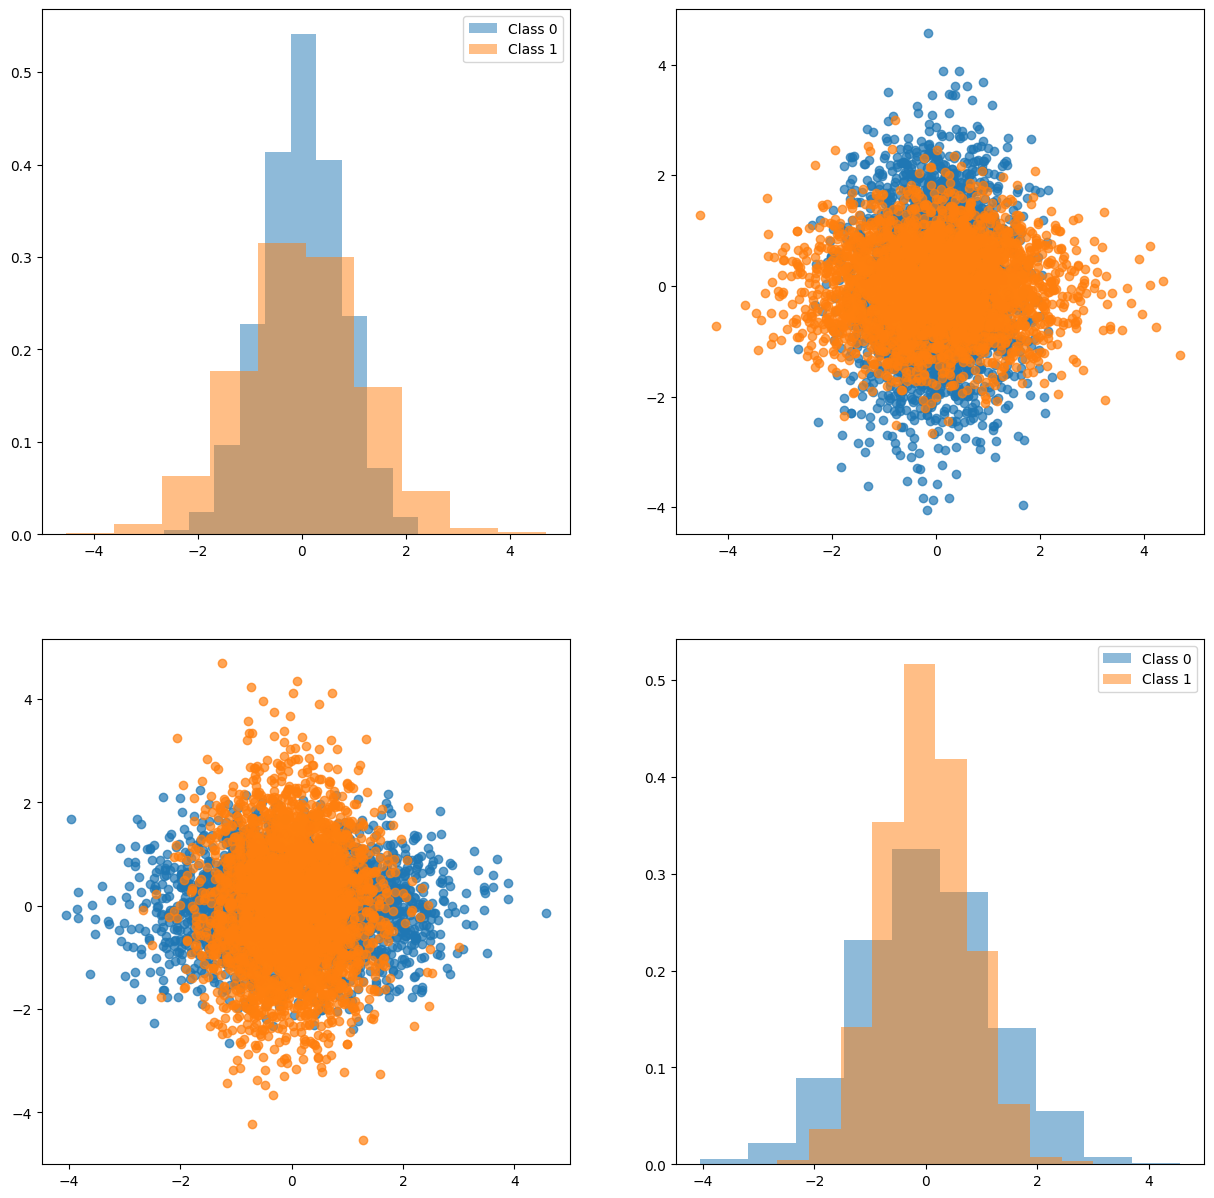
\includegraphics[width=\textwidth]{images/dataset_12.png}
        \caption{Features 1 and 2.}
    \end{subfigure}
    \hfill
    \begin{subfigure}[b]{0.3\textwidth}
        \centering
        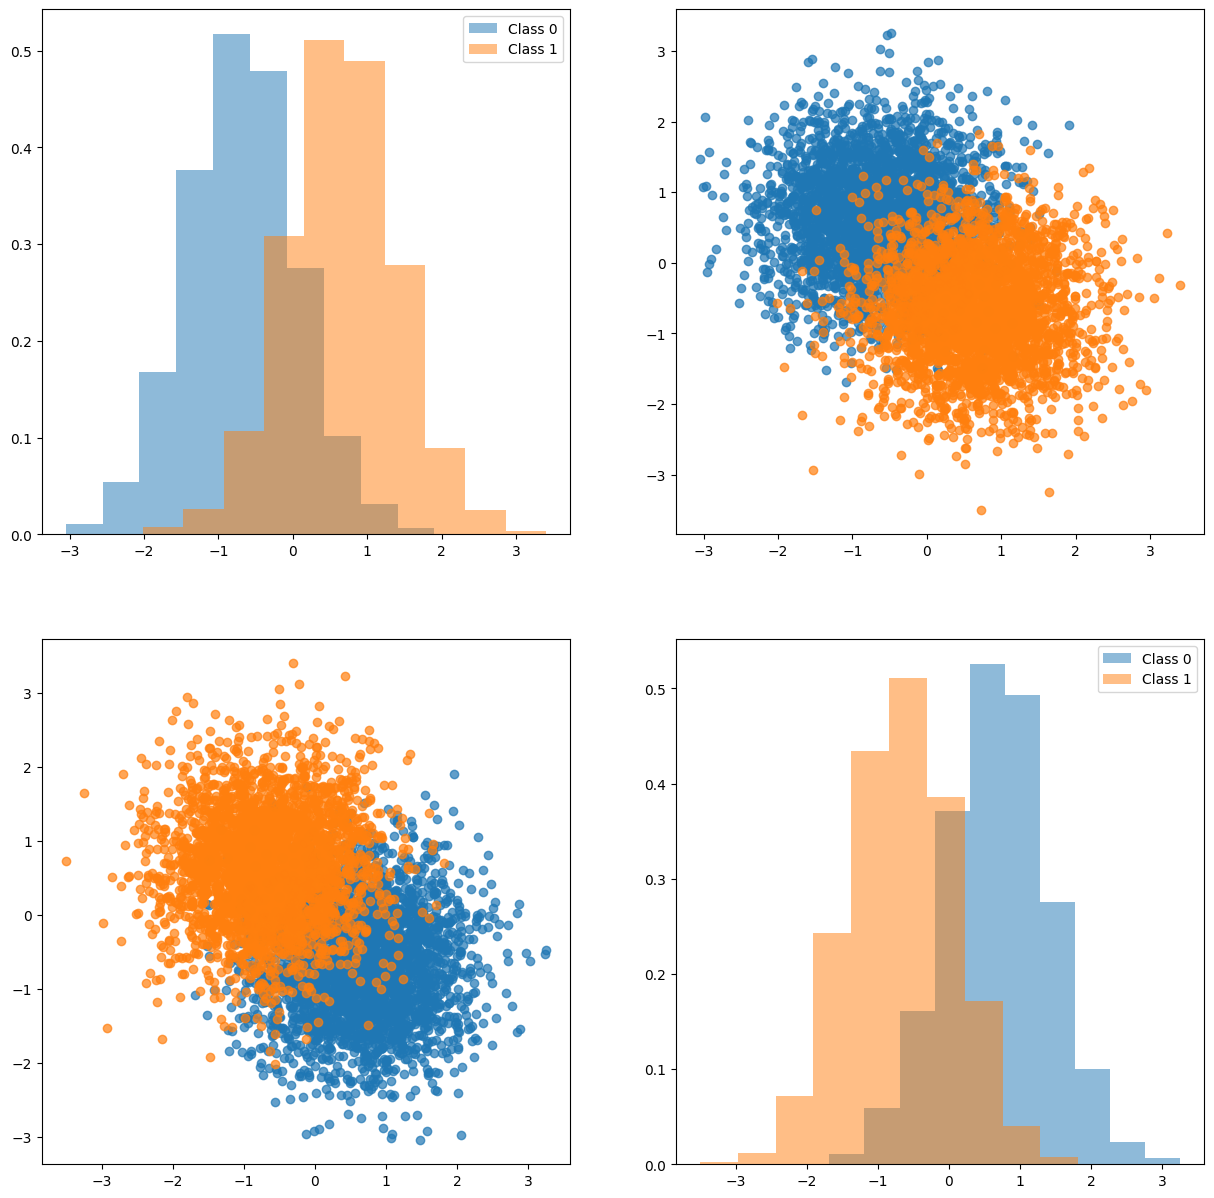
\includegraphics[width=\textwidth]{images/dataset_34.png}
        \caption{Features 3 and 4.}
    \end{subfigure}
    \hfill
    \begin{subfigure}[b]{0.3\textwidth}
        \centering
        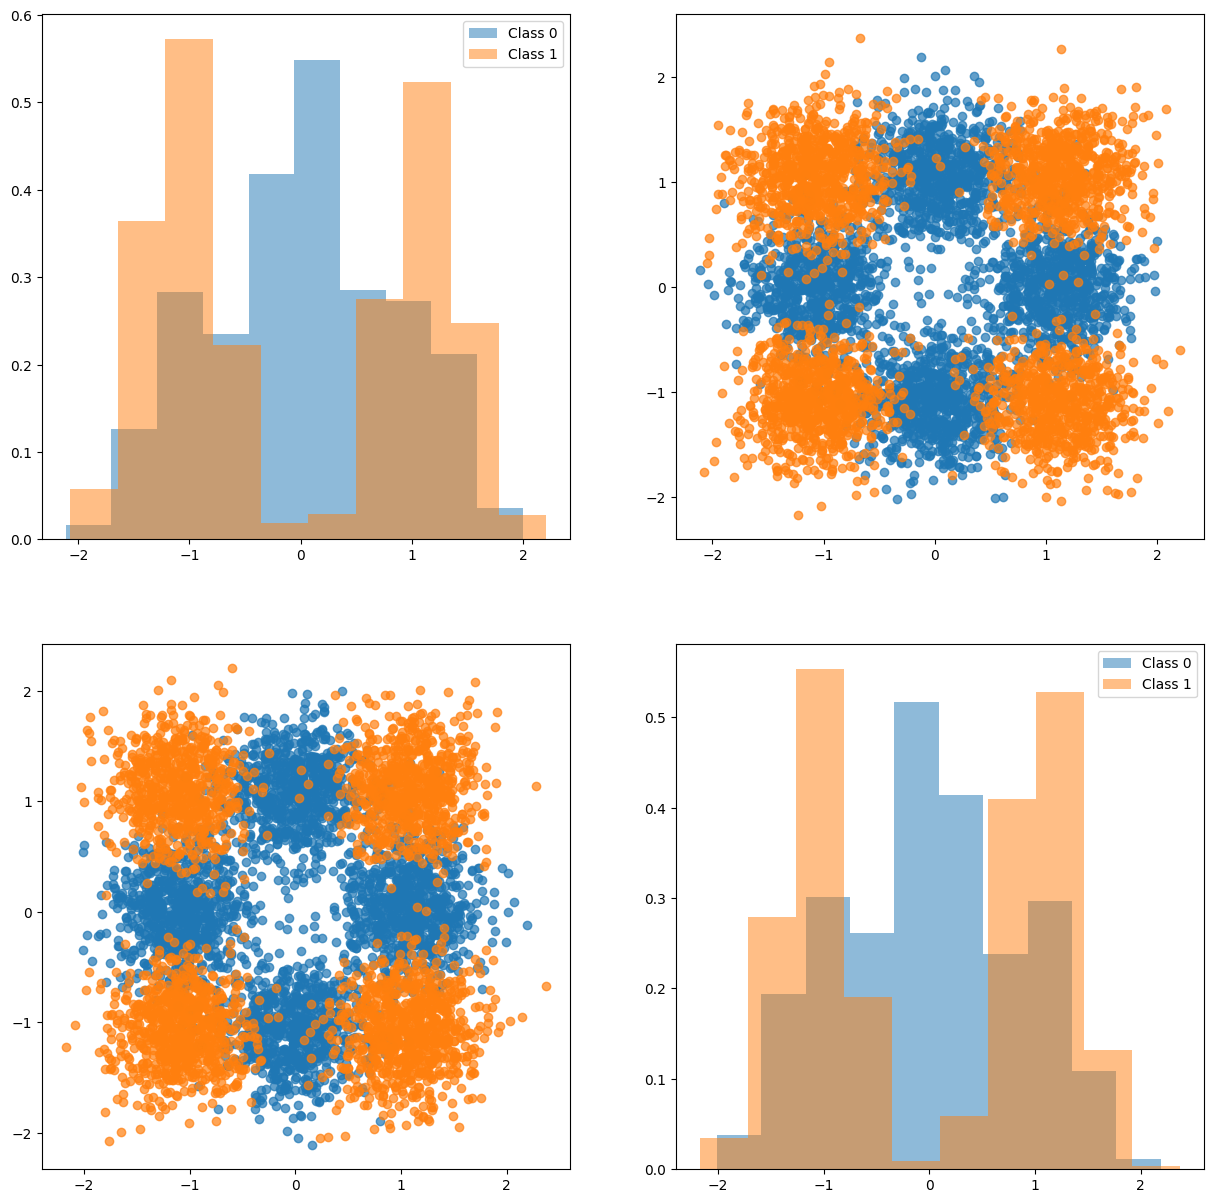
\includegraphics[width=\textwidth]{images/dataset_56.png}
        \caption{Features 5 and 6.}
    \end{subfigure}
    \caption{The figure shows histograms of the projected data on each feature. The scatter plot shows the correlation between the two features.}
    \label{fig:dataset}
\end{figure}

The first two features are mostly overlapping, so it is difficult to separate the two classes. The histograms show that they can be probably well approximated by a Gaussian density function. Further more means are very close to each other and only the second feature has a slightly difference in variance. 

The third and fourth features are more separated, but still overlapping. Also these features can be approximated by a Gaussian density function but the means are different and variance very similar. These features are more useful in a classification task as they are more discriminative.

The last two features are the most discriminative, they can't be approximated by a simple unimodal Gaussian density function because they seems to be bimodal. Thanks to this behavior they form 4 distinct clusters (two for each feature) that can be easily separated. They are probably the most useful features if the classifier is able to capture the complex structure.

\section{Lab 3: PCA and LDA}
\label{sec:pca_lda}

\subsection{Dimensionality Reduction}

\begin{figure}[ht]
    \centering
    \includegraphics[width=\textwidth]{images/dataset_pca.png}
    \caption{The figure shows the results of PCA on the dataset. The histograms show data distribution on each principal component. The top left one represents the first principal component, the bottom right is the last one. }
    \label{fig:dataset_pca}
\end{figure}

Principal Component Analysis (PCA) is a dimensionality reduction technique that finds the directions of maximum variance in the data. It projects the data onto a lower-dimensional subspace while preserving as much variance as possible.
The Figure \ref{fig:dataset_pca} shows the results of PCA on the dataset. The first principal component captures most of the variance and it separates decently the two classes. The other principal components overlap, so they are not very useful for classification.

\begin{figure}[ht]
    \centering
    \includegraphics[width=\textwidth]{images/dataset_lda.png}
    \caption{The figure shows the results of LDA on the dataset. The histogram shows data distribution on the only linear discriminant found.}
    \label{fig:dataset_lda}
\end{figure}

Linear Discriminant Analysis (LDA) is a supervised dimensionality reduction technique that finds the directions that maximize the separation between classes. 
The Figure \ref{fig:dataset_lda} shows the results of LDA on the dataset. Only one linear discriminant is found because the number of classes is 2. The linear discriminant separates the two classes partially. It is comparable to the first principal component of PCA.

Both cases simplify the dataset as much that the well-distinctive cluster of the last two features is lost. So, the preprocessing techniques cloud be useful to speed up the computation but they could also lose important information. In very simple dataset ad this one, with only 6 dimensions, presumably the best choice is to use the original dataset.

\subsection{Classification}
The project analyses the performance of LDA method as a classifier. In order to get reliable results, the experiments' performance is evaluated with k-fold cross-validation with k equal to 10. It is also inspect the improvement of the classifier by using PCA as a preprocessing technique.

The Table \ref{tab:lda_performance} shows the performance results as error rate, Detection Cost Function (DCF) and Minimum DCF. The last one is useful to understand the gains of changing the threshold to optimal value.

\begin{table}[ht!]
    \centering
    \begin{tabularx}{\textwidth}{lXXX}
        \toprule
        \textbf{PCA} & \textbf{Error Rate (\%)} & \textbf{DCF} & \textbf{Min DCF} \\
        \midrule
        None   & 9.58 & 0.192 & 0.176 \\
        1 PC  & 9.68 & 0.194 & 0.177 \\
        2 PC  & 9.63 & 0.193 & 0.178 \\
        3 PC  & 9.43 & 0.189 & 0.176 \\
        4 PC  & 9.57 & 0.192 & 0.175 \\
        5 PC  & 9.58 & 0.192 & 0.175 \\
        6 PC  & 9.62 & 0.193 & 0.176 \\
        \bottomrule
    \end{tabularx}
    \caption{Performance metrics for LDA models with various dimensionality reduction techniques.}
    \label{tab:lda_performance}
\end{table}

As intuitively retrieved from PCA and LDA graphs, the capabilities of both methods are similar. In fact, the performance of the classifier is not improved by using PCA as a preprocessing technique. 

In general the performance are terrible considering the simplicity of the dataset. Further more the threshold selection is not optimal, so the performance could be improved by tuning it a little bit.

\section{Lab 4: Multivariate Gaussian density}
\label{sec:multivariate_gaussian}
Describe the methods used in your project. Include algorithms, data preprocessing steps, feature selection, model selection, and any other relevant details.

\subsection{Data Collection and Preprocessing}
Detail the data sources, collection methods, and preprocessing steps.

\subsection{Algorithm and Model Selection}
Discuss the algorithms and models used. Include any hyperparameter tuning and model selection processes.

\subsection{Evaluation Metrics}
Explain the metrics used to evaluate the performance of your models.

\section{Experiments}
\label{sec:experiments}
Describe the experiments conducted to validate your models. Include details such as experimental setup, datasets used, and any specific configurations.

\section{Results}
\label{sec:results}
Present the results of your experiments. Use tables, figures, and charts to illustrate the performance of your models.

\begin{table}[ht]
    \centering
    \begin{tabular}{|c|c|c|}
        \hline
        Model & Accuracy & F1 Score \\
        \hline
        Model 1 & 0.90 & 0.88 \\
        Model 2 & 0.85 & 0.84 \\
        Model 3 & 0.92 & 0.90 \\
        \hline
    \end{tabular}
    \caption{Model performance comparison}
    \label{tab:results}
\end{table}

\section{Discussion}
\label{sec:discussion}
Interpret the results. Discuss any patterns, insights, or anomalies observed. Compare the performance of different models and explain any differences.

\section{Conclusion}
\label{sec:conclusion}
Summarize the findings of your project. Discuss the implications of your results, any limitations of your study, and possible future work.

\end{document}
